\section{Othello}
\label{sec:othello}

Othello ist ein Spiel für zwei Spieler, in dem es darum geht, zum Ende des Spiels möglichst viele Steine der eigenen
Farbe auf dem Spielfeld, einem $8\times 8$ Felder großem quadratischen Gitter, liegen zu haben.

\begin{figure}[H]
    \centering
    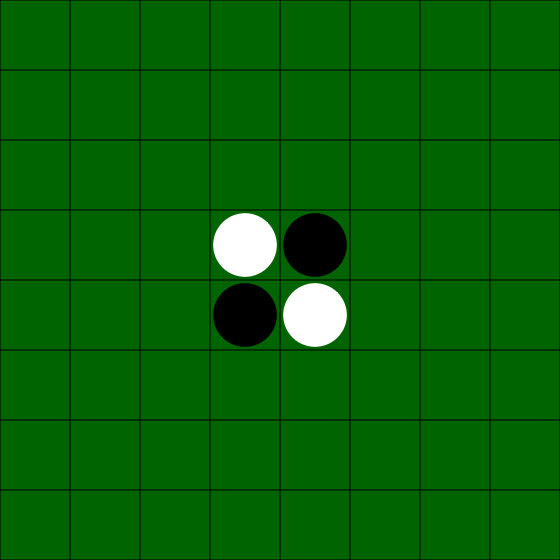
\includegraphics[width=\textwidth / 2]{board_initial}
    \caption{Initialer Spielzustand}
    \label{fig:board_initial}
\end{figure}

Zu Beginn des Spiels liegen auf den vier mittleren Feldern des Spielfelds jeweils zwei Steine jedes Spielers so, dass
wie in Abbildung \ref{fig:board_initial} zu sehen ist, die Steine eines Spielers einander diagonal gegenüber liegen.

Die Spieler legen nun abwechselnd jeweils einen Stein ihrer eignen Farbe auf das Spielfeld. Steine können nur auf freie
Felder gelegt werden, die in horizontale, vertikale oder diagonale Richtung an einen oder mehrere gegnerische Steine,
gefolgt von einem eigenen Stein, angrenzen. Eine beispielhafte Spielsituation, in der die möglichen Spielzüge für den
schwarzen Spieler als kleinere Scheiben dargestellt werden, ist in Abbildung \ref{fig:board_possible_moves} zu sehen. 

\begin{figure}[H]
    \centering
    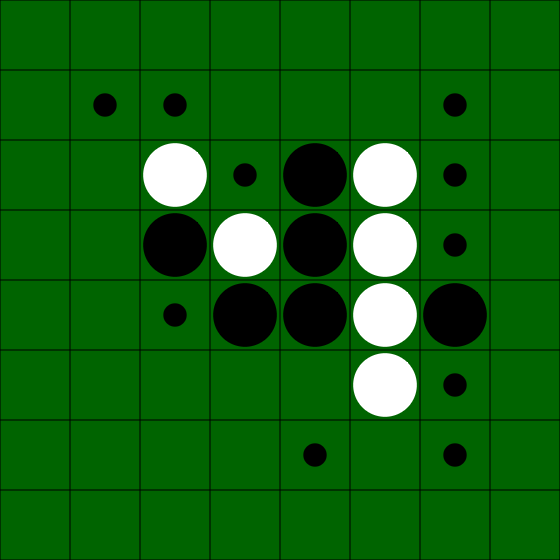
\includegraphics[width=\textwidth / 2]{board_possible_moves}
    \caption{Mögliche Züge des schwarzen Spielers}
    \label{fig:board_possible_moves}
\end{figure}

Alle gegnerischen Steine, die durch den gesetzten Stein in eine der 8 Richtungen lückenlos, d. h. ohne freie Felder
dazwischen, eingeschlossen werden, werden umgedreht und ändern dadurch ihre Farbe zu der des anderen Spielers.

Ist einer der Spieler zugunfähig, das heißt, er ist an der Reihe, kann jedoch keinen validen Zug spielen, so ist der
andere Spieler erneut am Zug.

Das Spiel endet, sobald beide Spieler zugunfähig sind. Der Gewinner ist dann der Spieler, der die meisten Steine seiner
Farbe auf dem Spielfeld liegen hat.
\cite{worldothellorules}
